\documentclass[12pt, openany]{report}
\usepackage[utf8]{inputenc}
\usepackage[T1]{fontenc}
\usepackage[a4paper,left=2cm,right=2cm,top=2cm,bottom=2cm]{geometry}
\usepackage[frenchb]{babel}
\usepackage{libertine}
\usepackage[pdftex]{graphicx}
\usepackage{amssymb}
\usepackage{listings}


\usepackage[colorlinks=true,linkcolor=red]{hyperref}
\usepackage[nottoc, notlof, notlot]{tocbibind}

\usepackage{cite}

\setlength{\parindent}{1cm}
\setlength{\parskip}{1ex plus 0.5ex minus 0.2ex}
\newcommand{\hsp}{\hspace{20pt}}
\newcommand{\HRule}{\rule{\linewidth}{0.5mm}}
\begin{document}

\begin{titlepage}
  \begin{sffamily}
  \begin{center}

    % Upper part of the page. The '~' is needed because \\
    % only works if a paragraph has started.
    
\includegraphics[scale=0.2]{Images/UMONS+txt.png}   ~\\[1.5cm]
    


    \HRule \\[0.4cm]
    { \huge \bfseries Projet de Software Evolution - JPacman\\[0.4cm] }
    \HRule \\[2cm]
    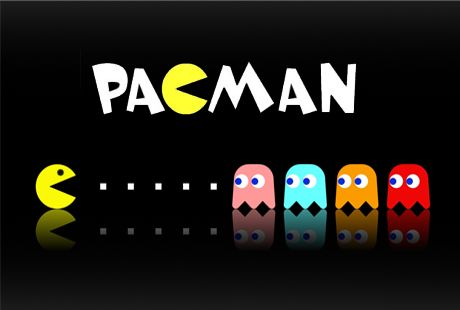
\includegraphics[scale=0.5]{Images/Pac-Man.jpg}~\\[1.5cm] 

    
    

    % Author and supervisor
    \begin{minipage}{0.4\textwidth}
      \begin{flushleft} \large
        \emph{Réalisateurs :\\} Damien \textsc{Legay}\\ Adrien \textsc{Coppens}\\ Nicolas \textsc{Leemans}\\
        
      \end{flushleft}
    \end{minipage}
    \begin{minipage}{0.4\textwidth}
      \begin{flushright} \large
        \emph{Enseignant :} M. Tom  \textsc{Mens}\\
        \emph{Date de remise : } 9 mai 2016\\
        \emph{Année d'étude : } Master 1
      \end{flushright}
    \end{minipage}

    \vfill

    % Bottom of the page
    {\large Année académique 2015 - 2016}
	
  \end{center}
  \end{sffamily}
\end{titlepage}




\newpage


	\tableofcontents
	\newpage
	\setcounter{secnumdepth}{3}
	\setcounter{tocdepth}{4}
	

\chapter{Introduction}

Ce projet, effectué dans le cadre du cours de "Software Evolution" dispensé par Monsieur Tom Mens durant l'année académique 2015-2016, a pour but de mettre en pratique les concepts d'évolution logicielles vus au cours théorique. Il consiste à analyser et à étendre un projet pour ensuite l'évoluer à l'aide de \textit{"refactorings"}. Le projet concerné s'appelle JPacman\footnote{https://github.com/SERG-Delft/jpacman-framework}. Il s'agit d'une implémentation très basique du jeu Pacman en Java, créé par l'équipe  du professeur Arie van Deursen, Delft University of Technology (Pays-Bas).
 JPacman contient plusieurs simplifications par rapport au jeu Pac-Man original. Le jeu consiste à déplacer Pac-Man, un personnage qui, vu de profil, ressemble à un diagramme circulaire à l’intérieur d’un labyrinthe, afin de lui faire manger toutes les pac-gommes qui s’y trouvent en évitant d’être touché par des fantômes.
 
 Ce rapport s'organise en plusieurs chapitres : dans un premier chapitre, ...
 
\chapter{Extension du projet et ajout de tests unitaires pour cette extension }

\section{Extension du logiciel}

La première partie de ce projet consistait à étendre la version initial de JPacman en ajoutant de nouvelles fonctionnalités et en suivant un processus de développement dirigé par les tests. De nouveaux tests unitaires ont donc été ajoutés pour chaque fonctionnalité afin de vérifier que le comportement initial du logiciel n’a pas été altéré. 

Chaque membre du groupe a donc implémenté une des fonctionnalités suivantes :
\begin{itemize}
\item L'implémentation d'un score (réalisé par Damien Legay)
\item L'implémentation d'une série de labyrinthes (réalisé par Adrien Coppens)
\item L'implémentation d'une intelligence artificielle pour pacman (réalisé par Nicolas Leemans)

\end{itemize}

\subsection{Fonctionnalité "Score"}
\subsection{Fonctionnalité "Série de labyrinthes"}
\subsection{Fonctionnalité "IA pour Pacman"}











\chapter{Refactorings avant analyse}
%todo: ce qui était prévu juste après merge, qu'on avait laissé tel quel ds les parties individuelles pr éviter au maximum les conflits lors de l'intégration des PR

\subsubsection{Fusion des tests sur \og Player \fg}
%Des tests avaient été effectués par 2 d’entre nous et lors de la fusion, nous avions simplement fusionné ceux-ci en ignorant la redondance de variables d’instances. L’un des 2 tests n’utilisant pas les \og mocks \fg, une légère adaptation a été nécessaire pour que le mock de fantôme retourne une valeur lors de l’appel à \og Ghost#getIdentity() \fg.
\subsubsection{Déplacement de la variable retenant le niveau courant de \og Level \fg vers \og Game \fg}
%Plus logique et évite un problème de \og feature envy \fg 
\subsubsection{Déplacement des méthodes concernant le \og map parser \fg de \og Launcher \fg vers \og Game \fg}
%Plus logique et évite que \og Game \fg doive avoir une référence vers le \og Launcher \fg qui l’a créé (pour pouvoir charger le niveau suivant en cas de \og victoire \fg)
%A nécessité de passer des méthodes/variables en \og static \fg (une partie des accesseurs aux \og Factories \fg de \og Launcher \fg puisque \og MapParser \fg en a besoin) mais cela reste logique puisque ces méthodes/variables sont en effet uniques au runtime.









\chapter{Analyse de la qualité du code source}

Dans ce chapitre, nous allons comparer la qualité du code source qui intègre toutes les extensions individuelles avec la qualité du code source de la version de départ de JPacman. Pour pouvoir effectuer cette comparaison, il va, tout d'abord, falloir effectuer des analyses sur la qualité du code source des deux versions en utilisant différents types d'analyses et de techniques. Pour effectuer cette analyse, nous ferons appel à plusieurs outils d'analyse de qualité que nous détaillerons par la suite. Cette phase d'analyse se déroulera en trois étapes : une analyse statique et dynamique du code ainsi qu'une analyse de la qualité par plusieurs métriques logicielles qui peuvent aider à déceler de mauvaises pratiques. 

\section{Analyse statique}
\subsection{Code dupliqué}
Puisque nous utilisons tous les 3 IntelliJ IDEA, l'outil intégré a été utilisé dans un premier temps. La figure \ref{duplicate} montre les résultats obtenus via cette analyse.
On peut noter que les détections ayant un \og coût \fg \, inférieur à $\sim$20 ne sont pas réellement préoccupantes. Pour exemple, les lignes suivantes, extraites de \textit{SquareCoordinateTest}, sont considérées comme dupliquées par l'outil avec un score de 10 :
\begin{lstlisting}[language=java]
assertEquals(square.getSquareAt(Direction.WEST).getY(), 15);
assertEquals(square.getSquareAt(Direction.EAST).getY(), 15);
\end{lstlisting}
Il s'agit en effet de 2 lignes très similaires mais il ne nous a pas semblé intéressant de supprimer ce type de duplicat. 
%todo: actions en réaction aux duplicats évitables et significatifs (coût > 25?)
Dans un second temps, nous avons analysé le code via \textit{CPD} inclus dans \textit{PMD} et qui était utilisé dans la suite de rapports à générer par \textit{Maven}. Le seul dupliqué signalé par cet outil concerne la classe \textit{AStarPathTest} pour laquelle les méthodes \textit{hTest} et \textit{gTest} contiennent en effet toutes deux ce bloc de code :
\begin{lstlisting}[language=java]
final AStarPath aStarPath = new AStarPath(game);

assertNotNull(aStarPath);
final Player player = game.getPlayers().get(0);
final Square square = player.getSquare();

assertNotNull(player);
assertNotNull(square);

final Square origin = player.getSquare();
final Square destination = player.getSquare().getSquareAt(Direction.EAST);
final Square destination2 = player.getSquare().getSquareAt(Direction.EAST).getSquareAt(Direction.EAST);

final Square destination3 = player.getSquare().getSquareAt(Direction.WEST);
final Square destination4 = player.getSquare().getSquareAt(Direction.WEST).getSquareAt(Direction.WEST);
\end{lstlisting}
%todo: action entreprise (extract method?)

\begin{figure}[h]
	\centering
	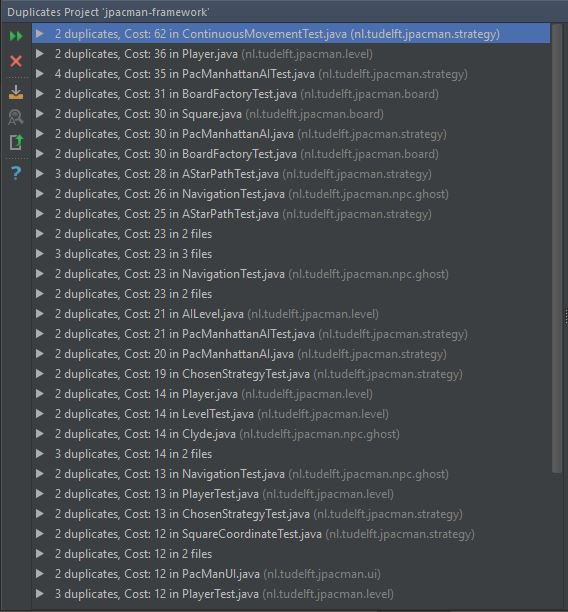
\includegraphics{Images/duplicate_analysis.JPG}
	\caption{\label{duplicate} Recherche de code dupliqué via l'outil intégré à \textit{IntelliJ IDEA}}
\end{figure}

\subsection{CheckStyle}
Egalement intégré dans la suite d'analyses à effectuer via \textit{Maven}, \textit{CheckStyle} a été utilisé avec le \og ruleset \fg \, présent dans la version du code d'origine.
Aucune erreur n'a été détectée mais de nombreux \og warnings \fg \, sont cependant présents (plus de 500). Par ordre de nombre de \og violations \fg :
\begin{itemize}
	\item 148 violations de type \textit{JavadocStyle} : en réalité toutes des \og First sentence should end with a period. \fg $\rightarrow$ réglé. 
	\item 110 violations de type \textit{MagicNumber} $\rightarrow$ constantes extraites là où cela avait du sens, sauf pour les tests où un tel refactoring nous semblait inutile, nous avons donc supprimé les \og warnings \fg \, pour ceux-ci.
	\item 104 violations de type \textit{LineLength} $\rightarrow$ retours à la ligne là où c'était nécessaire.
	\item 63 violations de type \textit{NeedBraces} $\rightarrow$ bien que nous ne soyons pas tous d'accord sur la valeur ajoutée d'une telle convention, nous avons ajouté les crochets là où \textit{CheckStyle} le demandait.
	\item 35 violations de type \textit{AvoidStarImport} $\rightarrow$ encore une fois désactivés car nous utilisons la fonction \og optimize imports \fg \, d'\textit{IntelliJ IDEA} qui regroupe parfois des imports en un unique via cette notation.
	\item Des violations relatives à des éléments de javadoc manquants $\rightarrow$ ajoutés.
	\item Des violations relatives à des tableaux déclarés à la \og mode C \fg \, plutôt qu' à la \og mode Java \fg $\rightarrow$ modifiés.
\end{itemize}

\subsection{IntelliJ Code inspection}
\subsubsection{IntelliJ dit que la condition impliquant QUICK\_WIN est \og pointless \fg} 
%Puisque la variable mise à true ou false dans le code, c’est effectivement le cas sur le code compilé, pas dans le code source puisqu’on veut pouvoir le changer. Note qu’on pourrait aussi permettre de set ça en paramètre au lancement du prog (option type \og --quick \fg)
\subsubsection{Changements mineurs (\og scope \fg de méthodes/variables, variables qui peuvent être \og final \fg)}
\subsubsection{Dans le code de base, beaucoup de \og warnings \fg sur des \og problèmes de modernité \fg}
%for indexé plutôt que foreach, méthode anonyme classique plutôt que lambda, etc

\subsection{PMD}
\subsubsection{Déplacement des méthodes liées à la récupération des cases \og safe \fg pour téléporter le joueur de Level vers Board}
%Plus logique et évite un problème de \og feature envy \fg desdites méthodes
\subsubsection{Problème détecté par PMD : Level == godclass}
%Signifie que :
%1.	Level a une \og cohésion interne \fg faible, nous sommes en effet très loin du seuil de 1/3 mais cela devait également être le cas dans la version de base
%2.	Level accède à des attributs appartenant à trop de classes étrangères, encore une fois, peu de changements à ce niveau là par rapport à la version de base
%3.	Level est \og trop complexe par rapport à sa taille \fg : le problème ici semble venir de PMD qui, d’après la règle définie sur https://pmd.github.io/pmd-5.4.1/pmd-java/xref/net/sourceforge/pmd/lang/java/rule/design/GodClassRule.html attribue effectivement une valeur de complexité mais à aucun moment ne prend en compte la \og taille \fg de la classe.
%Etant donné que Level comprend beaucoup de méthodes, la complexité est naturellement élevée.


\section{Analyse dynamique}
\section{Mesure de la qualité du logiciel}
\section{Conclusion de l'analyse}





%\bibliographystyle{plain}
%\bibliography{bibliographie}
\end{document}